% !TeX program = lualatex
\documentclass[11pt]{beamer}
\usefonttheme[onlymath]{serif}
\usepackage[utf8]{inputenc}
\usepackage[T1]{fontenc}
\usepackage{bbm}
\usepackage{lmodern}
% \usepackage[hidelinks]{hyperref}
\usepackage[autolanguage]{numprint}
\usepackage[utf8]{inputenc}
\usepackage[T1]{fontenc}
\usepackage[french]{babel}
\usepackage{graphicx}
\graphicspath{{./fig/}}
\usepackage{listings}
\usepackage{pgfpages}

%\setbeameroption{show notes on second screen=right} %for ds pdf viewer

\usepackage{fontawesome} %font fa logo

\usepackage{color}
\definecolor{dkgreen}{rgb}{0,0.6,0}
\definecolor{gray}{rgb}{0.5,0.5,0.5}
\definecolor{mauve}{rgb}{0.58,0,0.82}

\lstset{ %
language=R,                     % the language of the code
basicstyle=\footnotesize,       % the size of the fonts that are used for the code
numbers=left,                   % where to put the line-numbers
numberstyle=\tiny\color{gray},  % the style that is used for the line-numbers
stepnumber=1,                   % the step between two line-numbers. If it's 1, each line
% will be numbered
numbersep=5pt,                  % how far the line-numbers are from the code
showspaces=false,               % show spaces adding particular underscores
showstringspaces=false,         % underline spaces within strings
showtabs=false,                 % show tabs within strings adding particular underscores
tabsize=4,                      % sets default tabsize to 2 spaces
captionpos=b,                   % sets the caption-position to bottom
%breaklines=true,                % sets automatic line breaking
breakatwhitespace=false,        % sets if automatic breaks should only happen at whitespace
title=\lstname,                 % show the filename of files included with \lstinputlisting;
% also try caption instead of title
keywordstyle=\color{blue},      % keyword style
commentstyle=\color{mauve},   % comment style
stringstyle=\color{dkgreen},      % string literal style
escapeinside={\%*}{*)},         % if you want to add a comment within your code
morekeywords={*,...}            % if you want to add more keywords to the set
} 

%% Renvois vers les scripts R
%%%%% Update color if name change
\newcommand{\gotoR}[1]{%
\begin{center}
	\colorbox{ulgold}{\color{black}
		\makebox[75mm][c]{%
			\makebox[5mm]{\raisebox{-1pt}{\large\faChevronCircleDown}}\;%
			{\ttfamily #1}}}
\end{center}}


\hypersetup{
colorlinks=true,
citecolor=blue,
linkcolor=black,
filecolor=magenta,
urlcolor=cyan,
}

\mode<presentation> {
\usetheme{ulaval}
\setbeamercovered{invisible}
}


\logo{%\includegraphics[height=0.6cm]{COPL}\hspace{.5cm}%

\includegraphics[height=1.5cm]{DotLayer_logo_short_COL_RVB}}%\hspace{.2cm}\vspace{.865\paperheight}}
\titlegraphic{

\includegraphics[height=1cm]{DotLayer_logo_full+tagline_COL_RVB}\vspace{0.7cm}

\includegraphics[height=1cm]{logo-universite-laval}\vspace{0.7cm}

\includegraphics[height=1cm]{crdm}\vspace{0.7cm}

\includegraphics[height=1cm]{graal}\vspace{0.7cm}
}

\title[Atelier pratique Git]{Bonnes pratiques \& Git}

%\subtitle{}

\author[D. Beauchemin]{David Beauchemin, BSc.}
\institute[.Layer]
{
.Layer, Université Laval, CRDM, GRAAL
}
\date{21 juin 2019} 

\AtBeginSection[]
{
\begin{frame}<beamer>
	\frametitle{Agenda}
	\tableofcontents[currentsection]
\end{frame}
}
\newenvironment{slide}[1]
{\begin{frame}[environment=slide]
	\frametitle{\insertsection \newline \large{#1}}}
{\end{frame}}

\usepackage{fontspec}

\setsansfont[Path=Muli/, BoldFont=Muli-Bold.ttf,
ItalicFont=Muli-Italic.ttf,
BoldItalicFont=Muli-BoldItalic.ttf]{Muli-Regular.ttf}%




\begin{document}

\begin{frame}[label=titre, plain]
	\titlepage
\end{frame}

\begin{frame}
	\begin{center}
		\begin{figure}
			
\includegraphics[width=0.75\linewidth,height=0.75\textheight,keepaspectratio]{git}
			\caption{https://xkcd.com/1597/}
		\end{figure}
	\end{center}
\end{frame}


\section[Introduction]{Introduction}


\begin{frame}{À propos}
	\begin{itemize}
		\item Membres de .Layer, une communauté ayant comme mission de promouvoir la collaboration et le partage de connaissances dans le domaine de la science des données.
		\item Organisation de conférence et d'atelier. 
	\end{itemize}
	\begin{center}
		\href{dotlayer.org}{dotlayer.org}\\
		
\includegraphics[height = 0.3cm]{facebook} : \href{https://www.facebook.com/MeetupMLQuebec/}{MeetupMLQuebec}
	\end{center}
\end{frame}

\begin{frame}{Objectifs}
	
	\begin{itemize}
		\item Développer des bonnes pratiques de travail.
		\item Apprendre à utiliser l'invite de commande.
		\item Apprendre à utiliser les commandes de bases de Git.
		\item Apprendre à utiliser les commandes plus avancées de Git.
	\end{itemize}
\end{frame}


\section[Ligne de commande]{Ligne de commande}


\begin{frame}{Ligne de commande}
	Pourquoi utiliser l'invite de commande ?
	\begin{itemize}
		\item<1-> Permet plus de flexibilité.
		\item<2-> Permet de comprendre ce que l'on fait.
		\item<3-> Permet d'en pratiquer l'utilisation.
		\item<4-> Permet d'avoir l'air plus \textit{élite}.
	\end{itemize}
\end{frame}


\begin{frame}[fragile]{Astuces}
	\begin{itemize}[<+->]
		\item Tab est votre amie!
		\item \verb|ctrl+r| pour faire une recherche dans les commandes antérieures.
		\item $\uparrow \downarrow$ pour naviguer dans les dernières commandes.
		\item \verb|man| pour afficher le manuel d'une fonction.
		\note{Pour Git bash command --help \href{https://github.com/swcarpentry/shell-novice/issues/249}{pour rajouter une commande similaire dans le shell.}}
	\end{itemize}
\end{frame}

\begin{frame}[fragile]{ls/la/ll}
	\begin{itemize}[<+->]
		\item \verb|ls| Permet d'afficher tous les fichiers et répertoires visibles.
		\item \verb|la| Agit comme \verb|ls| mais affiche en plus les fichiers et répertoires cachés.
		\item \verb|ll| permet d'afficher la taille des fichiers et répertoires visibles.
	\end{itemize}
\end{frame}

\begin{frame}[fragile]{cd \& pwd}
	\begin{itemize}[<+->]
		\item \verb|cd dir_name| permet de se déplacer dans un répertoire.
		\item \verb|cd ..| permet de remonter d'un répertoire. 
		\item \verb|cd| permet de remonter à la racine.
		\item \verb|pwd| permet de connaitre son emplacement actuel.
	\end{itemize}
\end{frame}

\begin{frame}[fragile]{mkdir \& rm}
	\begin{itemize}[<+->]
		\item \verb|mkdir| permet de créer un répertoire.
		\item \verb|touch| permet de créer un fichier vide.
		\item \verb|mkdir -p| permet de créer un répertoire et ses parents.
		\item \verb|rm| permet de supprimer un fichier.
		\item \verb|rm -fr| permet de supprimer un répertoire.
	\end{itemize}
\end{frame}

\begin{frame}[fragile]{mv \& cp}
	\begin{itemize}[<+->]
		\item \verb|mv| permet de renommer/déplacer un fichier ou répertoire.
		\item \verb|cp| permet de copier-coller un fichier ou un répertoire.
	\end{itemize}
\end{frame}

\begin{frame}{Exercice}
	Pour mettre en pratique les commandes, nous allons naviguer avec l'invite de commande pour créer un répertoire GitHub qui va contenir l'ensemble des répertoires git. 
	
	\begin{itemize}
		\item On débute en affichant les répertoires locaux.
		\item On se déplace dans l'endroit qu'on souhaite avoir le répertoire (selon votre discrétion).
		\item On crée le répertoire.
	\end{itemize}
\end{frame}

\begin{frame}[fragile]{Vim}
\begin{block}{Comment quitter Vim ?}
\begin{lstlisting}
Esc - :q
\end{lstlisting}
\end{block}
Comment configurer un autre éditeur de texte ?
\newline
\begin{center}
\href{https://stackoverflow.com/questions/2596805/how-do-i-make-git-use-the-editor-of-my-choice-for-commits}{Stack Overflow
}
\end{center}
\end{frame}

\begin{frame}[fragile]{SSH}
	Les serveurs de calcul fonctionnent habituellement en invite de commande. Pour communiquer avec eux on peut, en autre, utiliser SSH.
	
	\begin{block}{Secure SHell (SSH)}
		Il s'agit d'un protocole de communication sécurisé pouvant être établi entre des ordinateurs. Ce protocole permet d'établir une session à distance sécurisée.
	\end{block}
\end{frame}

\begin{frame}[fragile]{SSH}
	\begin{block}{}
		\verb|ssh davidbeauchemin@132.203.120.91|
	\end{block}
\end{frame}

\begin{frame}[fragile]{SSH - config}
Configuration d'identifiant de connexion SSH pour un serveur de calcul distant.
\bigskip

\begin{block}{Éditer le fichier  $\sim$/.ssh/config}
\begin{lstlisting}
Host {credential_name}
	Hostname {ip_address}
	User {username}
\end{lstlisting}
\end{block}
\end{frame}

\begin{frame}[fragile]{Astuces SSH}
	\begin{itemize}[<+->]
		\item \verb|ssh {hostname}|
		\item \verb|ssh-copy-ip {hostname}|
		\note{Permet de partager votre clé SSH avec le remote pour éviter d'avoir à écrire votre mot de passe à chaque connexion.}
		\item \verb|ssh -L {port_local}:localhost:{port_remote} {host}| 
		\note{Permet de binder votre port local avec le port d'une remote. Parfait pour ouvrir des jupyter notebook qui roule sur le remote en localhost browser.}
	\end{itemize}
\end{frame}

\begin{frame}[fragile]{Transferer des fichiers}
	\begin{itemize}[<+->]
		\item \verb|scp {remote}:{files_path} {local_path}|
		\note{Bilatéral suffit inverser l'ordre}
		\item \verb|scp -r {local_directory}:{remote} {path}|
		\note{Pour envoyer un directory.}
		\item \verb|scp -r {remote}:'{path}{pattern}' {local_path}| 
		\note{On peut aussi utiliser des regex.}	
	\end{itemize}
\end{frame}

\begin{frame}[fragile]{SCP - REGEX}
\begin{block}{Example}
\begin{lstlisting}
scp -r deepnlp:'/mnt/cnn_dm/model_1/*.png' Result
\end{lstlisting}
\end{block}
\end{frame}

\begin{frame}[fragile]{Autres outils intéressants}
	\begin{itemize}
		\item tmux
		\item cURL
		\item tail -f
		\item ZSH
		\item Oh-My-ZSH
		\item crontab/systemd
	\end{itemize}
\end{frame}


\section{Git}


\begin{frame}{Pourquoi faire du versionnage}
	\begin{itemize}[<+->]
		\item Permet de suivre les changements pour un ensemble de fichiers.
		\note{Delta modification}
		\item Permet de revenir à des versions antérieures du code.
		\item Permet de comparer les changements.
	\end{itemize}
\end{frame}

\begin{frame}{Nomenclature}
	\begin{itemize}
		\item Dépôt (repository)
		\item Commit
		\item Branche (branch)
		\item master
		\item Local = Votre ordinateur
		\item Remote = GitHub/GitLab
	\end{itemize}
	\note{La majorité des opérations de versionnages sont locales, c'est-à-dire effectuer à même votre ordinateur. Un utilisateur pourrait uniquement utiliser Git localement. Par contre, pour permettre la distribution et la \textit{sauvegarde} on utilise un remote. Il s'agit d'un drive mais supportant Git et offrant parfois des fonctionnalités.}
\end{frame}

\begin{frame}{Inspiration}
\centering
\href{https://git-scm.com/book/en/v2}{Pro Git} \\
\href{https://rachelcarmena.github.io/2018/12/12/how-to-teach-git.html}{How to teach Git}
\end{frame}

\begin{frame}{Environnement}
	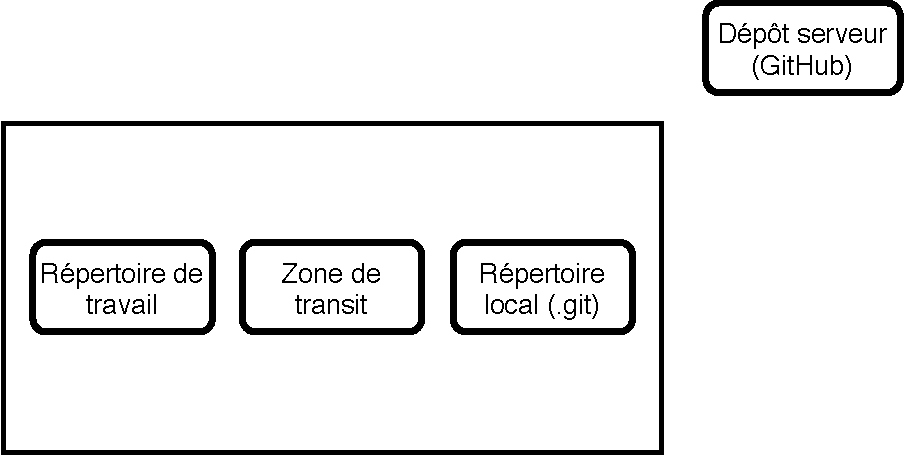
\includegraphics[width=0.95\linewidth,height=0.95\textheight,keepaspectratio]{env.pdf}
	\note{Git est un système de contrôle de version distribué. Cela signifie que chacun possède une version dans un état X du code. Git permet ainsi de gérer les versions avec un serveur distant.}
\end{frame}

\begin{frame}[fragile]
	Le plus simple pour partir un dépôt git est de créer un dépôt sur GitHub et de faire un \verb|git clone <url>|.
	
	\begin{itemize}[<+->]
		\item Initialize le dépôt,
		\item initialise les remotes,
		\item   s'initialise avec des fichiers de base automatiquement.
	\end{itemize}
\end{frame}

\begin{frame}{Cloner un répertoire}
	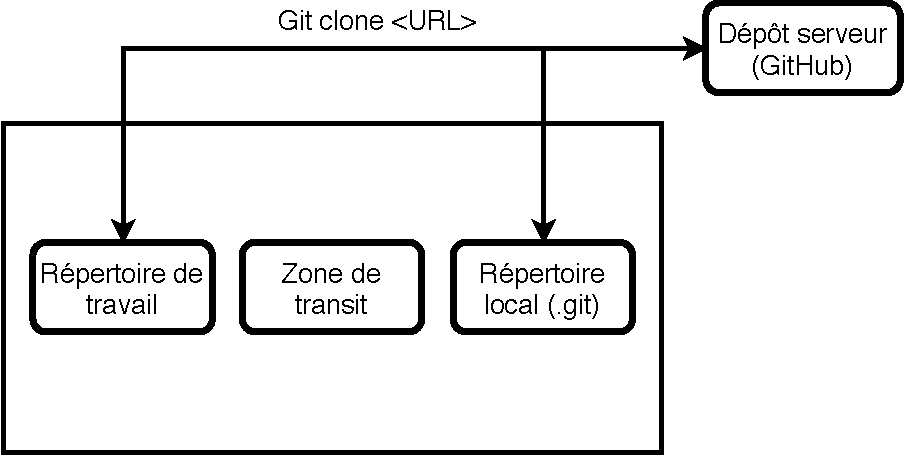
\includegraphics[width=0.95\linewidth,height=0.95\textheight,keepaspectratio]{clone.pdf}
\end{frame}

\begin{frame}{Exercice}
	\begin{block}{Cloner un dépôt}
		Aller cloner le dépôt de la formation \url{https://github.com/davebulaval/bonnes-pratiques-git.git}
	\end{block}
\end{frame}

\begin{frame}{Modification locale}
	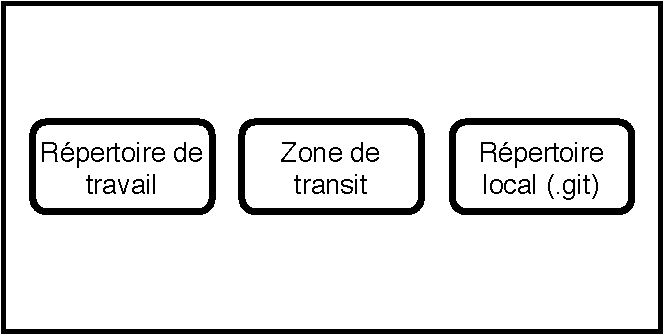
\includegraphics[width=0.95\linewidth,height=0.95\textheight,keepaspectratio]{stage.pdf}
\end{frame}


\begin{frame}{Modification locale}
	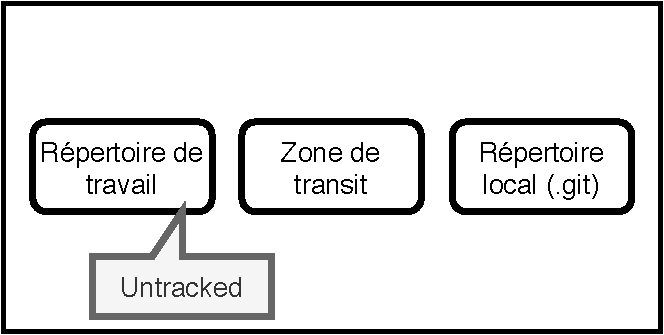
\includegraphics[width=0.95\linewidth,height=0.95\textheight,keepaspectratio]{untracked.pdf}
	\note{untracked : jamais commit.}
\end{frame}

\begin{frame}{Modification locale}
	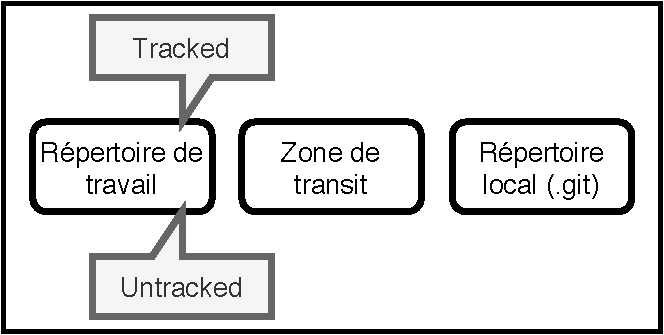
\includegraphics[width=0.95\linewidth,height=0.95\textheight,keepaspectratio]{modif.pdf}
	\note{Tracked: fichier déjà commit avec git.}
\end{frame}

\begin{frame}[fragile]{Modification locale}
	Avec Git, il est possible de facilement consulter l'état de notre environnement de travail. 
	\begin{itemize}
		\item Avec \verb|git status| il est facile de connaitre l'état des fichiers suivis et non suivis.
	\end{itemize}
\end{frame}

\begin{frame}{Zone de transit}
	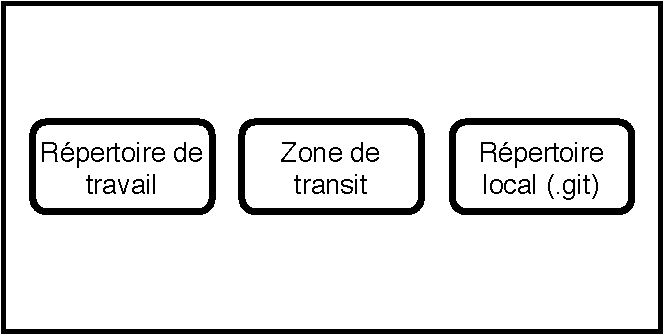
\includegraphics[width=0.95\linewidth,height=0.95\textheight,keepaspectratio]{stage.pdf}
\end{frame}

\begin{frame}{Zone de transit}
	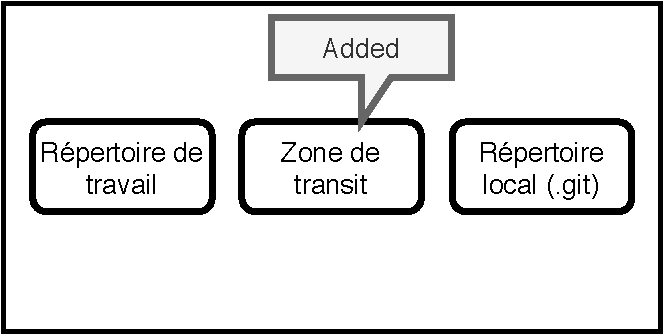
\includegraphics[width=0.95\linewidth,height=0.95\textheight,keepaspectratio]{added.pdf}
\end{frame}

\begin{frame}[fragile]{\textit{add} this}
	Pour préparer un commit, on doit indiquer à Git les fichiers que celui-ci doit contenir. Pour cela on passe par la zone de transit à l'aide de la commande \verb|git add|.
	
	\begin{itemize}[<+->]
		\item \verb|git add {fichiers}|
		\note{Permets de sélectionner les fichiers à ajouter manuellement.}
		\item \verb|git add -u|
		\note{Permets de sélectionner TOUS les fichiers suivis (donc modifier).}
		\item \verb|git add .|
		\note{Permets d'ajouter les fichiers suivis et non suivis.}
		\item \verb|git add -A|
		\note{Permets d'ajouter les fichiers suivis et non suivis en plus des fichiers supprimés.}
	\end{itemize}
\end{frame}

\begin{frame}{\textit{Workflow} \textit{git add}}
	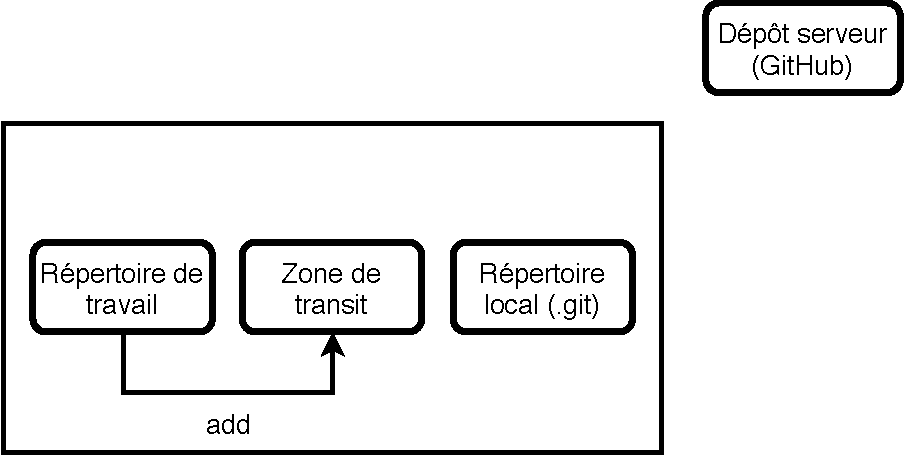
\includegraphics[width=0.95\linewidth,height=0.95\textheight,keepaspectratio]{add.pdf}
\end{frame}

\begin{frame}{Répertoire local}
	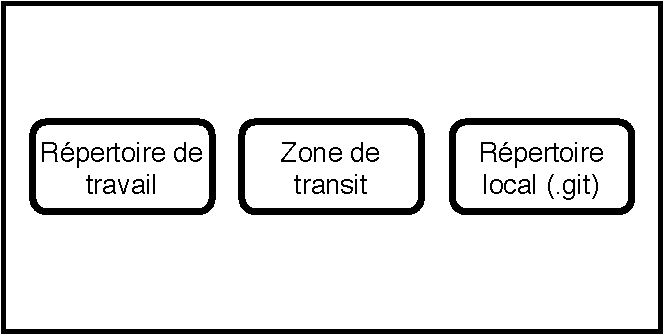
\includegraphics[width=0.95\linewidth,height=0.95\textheight,keepaspectratio]{stage.pdf}
\end{frame}

\begin{frame}{Répertoire local}
	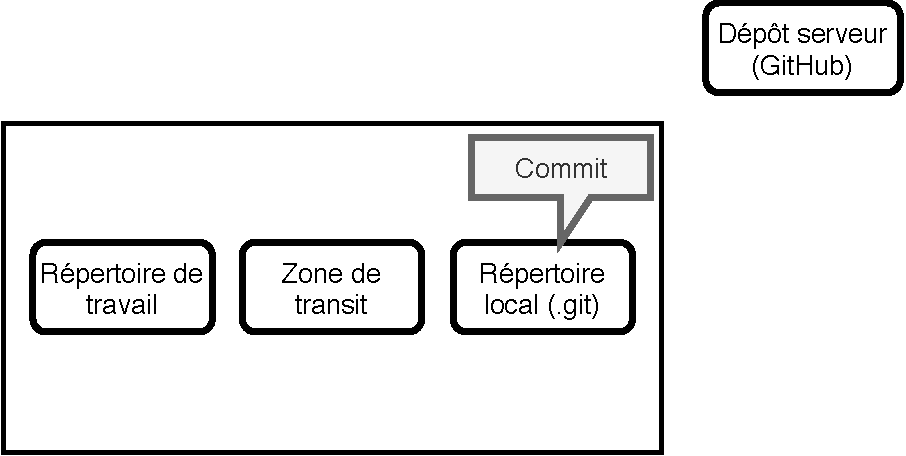
\includegraphics[width=0.95\linewidth,height=0.95\textheight,keepaspectratio]{commited.pdf}
\end{frame}

\begin{frame}[fragile]{\textit{commit} that}
	Lorsqu'on crée un commit, on prend un \textit{snapshot} de l'état du code à un moment $t$. Un commit  contient un titre et peut aussi contenir un contenu plus exhaustif.
	\bigskip
	
	Pour créer cela, on utilise la commande \verb|git commit|.
	
	\begin{itemize}[<+->]
		\item \verb|git commit|
		\note{Ouvre un éditeur interactif pour}
		\item \verb|git commit -m "message"|
		\note{Permets de commiter les fichiers stager avec le message.}
		\item \verb|git commit -a -m "message"|
		\note{Un git add-u suivie d'une git commit -m avec message.}
		\item \verb|git commit -m "message" --dry-run|
		\note{Permets de faire un semblant du commit pour vérifier que c'est bien ce que vous voulez faire.}
	\end{itemize}
\end{frame}
\begin{frame}{\textit{Workflow} \textit{git commit}}
	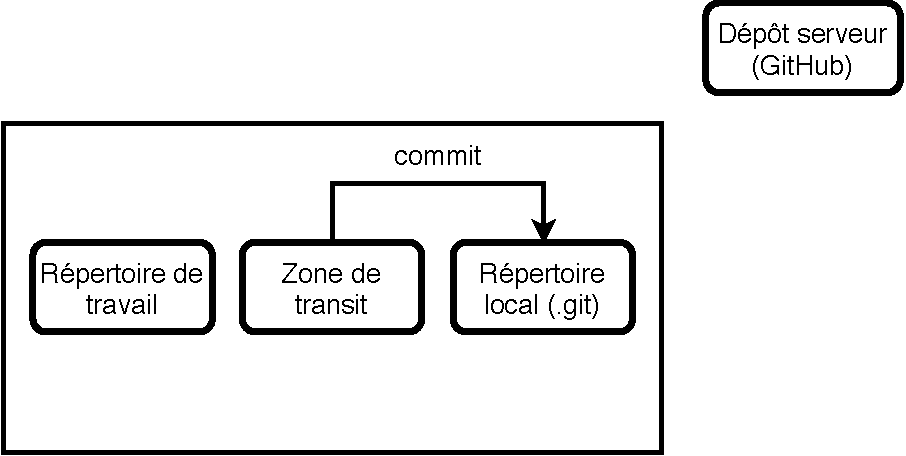
\includegraphics[width=0.95\linewidth,height=0.95\textheight,keepaspectratio]{commit.pdf}
\end{frame}

\begin{frame}[fragile]{\textit{diff} then}
	Jusqu'à présent, toutes ces étapes compliquées ne semblent pas apporter grand-chose. On ajoute des fichiers dans une zone de transit pour ensuite \textit{figer} les fichiers dans cette zone. On pourrait très bien avoir un nommage des versions. 
	\begin{itemize}
		\item rapport\_1.pdf
		\item rapport\_final.pdf
		\item rapport\_final-2.pdf
		\item code\_final-2\_final\_vrai.py
	\end{itemize}
\end{frame}

\begin{frame}[fragile]{\textit{diff} then}
	C'est la que \verb|git diff| entre en jeu. Avec cette commande, on est en mesure, \textit{ligne par ligne}, de voir les lignes de codes modifier. Ainsi, on est en mesure de savoir les deltas entre chaque version du code.
	\begin{itemize}[<+->]
		\item \verb|git diff|
		\note{Permets de faire un diff sur l'ensemble des fichiers du dépôt}
		\item \verb|git diff nom_fichier|
		\note{Permets de faire un diff sur un seul fichier}
		\item \verb|git diff --staged|
		\note{Permets de faire un diff sur les fichiers dans la zone de transit.}
		\item \verb|git diff commit hash_number|
		\note{Permets de faire un diff avec un commit précis.}
	\end{itemize}
\end{frame}

\begin{frame}{\textit{Workflow} \textit{git add; git commit}}
	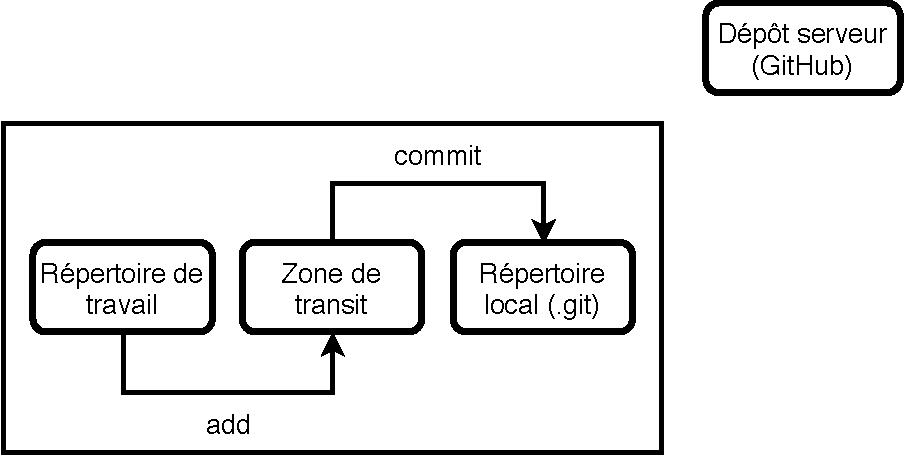
\includegraphics[width=0.95\linewidth,height=0.95\textheight,keepaspectratio]{add_commit.pdf}
\end{frame}

\begin{frame}[fragile]{Exercice}
	\begin{block}{\textit{Workflow}}
		Ajouter et modifier un fichier dans le répertoire cloner. \\
		Commiter uniquement le fichier modifier. \\
		Commiter le nouveau fichier.  \\
	\end{block}
	\textbf{Note:} Tenter d'utiliser les commandes \verb|git status| et \verb|git diff| tout au long du processus pour valider les actions prises.
\end{frame}

\begin{frame}[fragile]{\textit{Remote}}
	Pour mettre à jour le serveur distant, il suffit de faire lui \textit{pousser} l'information avec la commande \verb|git push|.
\end{frame}

\begin{frame}{\textit{Workflow} \textit{git add; git commit; git push}}
	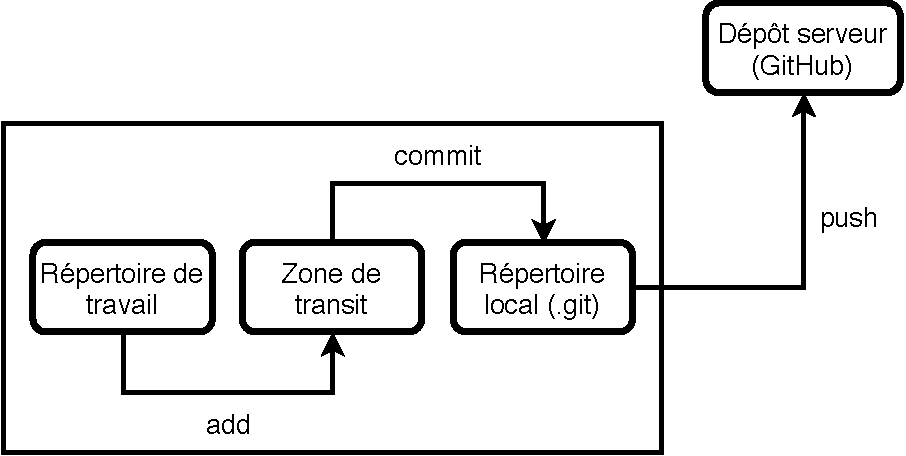
\includegraphics[width=0.95\linewidth,height=0.95\textheight,keepaspectratio]{workflow.pdf}
\end{frame}

\begin{frame}[fragile]{\textit{Remote}}
	Pour \textbf{se} mettre à jour avec le serveur distant, il suffit de lui \textit{demander} l'information avec la commande \verb|git pull|.
\end{frame}

\begin{frame}{\textit{Workflow} \textit{git pull}}
	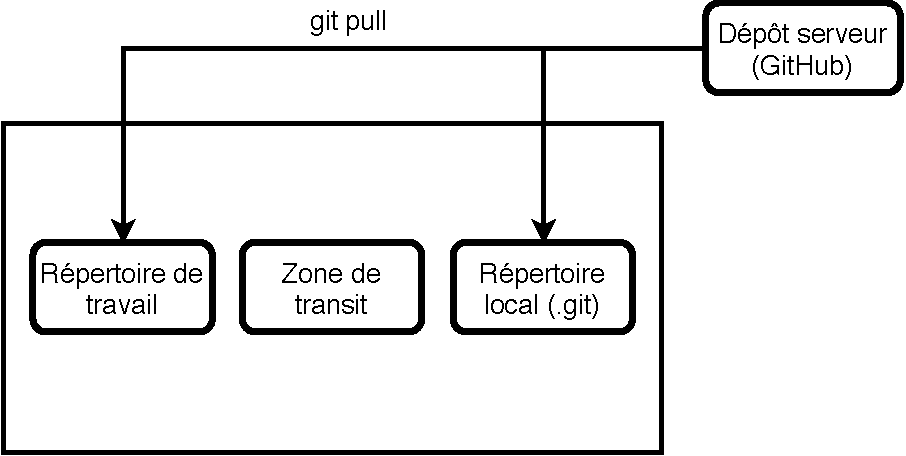
\includegraphics[width=0.95\linewidth,height=0.95\textheight,keepaspectratio]{pull.pdf}
\end{frame}

\begin{frame}[fragile]{Exercice}
	\begin{block}{\textit{Push}}
		Pousser les modifications au serveur. \\
	\end{block}
\end{frame}

\begin{frame}[fragile]{\textit{Remote}}
	Vous ne pouvez pas \verb|git push| si le serveur distant détecte qu'il vous manque des commits. Il faudrait alors faire un \verb|git pull| et potentiellement régler un \verb|merge conflict|.
\end{frame}

\begin{frame}[fragile]{Merge}
Si Git n'arrive pas à résoudre les conflits de fusion, il va vous indiquer dans le code source les endroits ou vous devez résoudre l'ambiguïté.
\begin{block}{}
\begin{lstlisting}
If you have questions, please
<<<<<<< HEAD
open an issue
=======
ask your question in IRC.
>>>>>>> branch-a
\end{lstlisting}
\end{block}
\end{frame}

\begin{frame}[fragile]{A branch for this and a branch for that!}
Un autre point qui distingue Git d'une utilisation simple de nommage est la possibilité de faire cohabiter plusieurs versions du code en même temps. Pour cela on utilise les branches.
	
	\begin{itemize}[<+->]
		\item \verb|git branch nom_branche|
		\note{Permets de créer une branche.}
		\item \verb|git branch -D nom_branche|
		\note{Permets de supprimer une branche.}
		\item \verb|git checkout nom_branche|
		\note{Permets de changer vers une branche existante.}
		\item \verb|git checkout -b nom_branche|
		\note{Permets de checkout sur une nouvelle branche.}
		\item \verb|git push --set-u origin nom_branche|
		\note{Pour configurer le upstream de votre nouvelle branche. Crée l'association.}
	\end{itemize}
\end{frame}

\begin{frame}{Exercice}
	\begin{block}{Créer une branche}
		Créer une branche. \\
		Ajoutez un fichier et mettez à jour le serveur. \\
	\end{block}
\end{frame}

\begin{frame}[fragile]{Fusionner des branches}
	L'intérêt d'avoir des branches est de pouvoir ensuite les fusionner. Pour cela, on utilise la commande \verb|git merge nom_branche|.
\end{frame}

\begin{frame}{Exercice}
	\begin{block}{Fusionner une branche}
		Fusionner votre branche avec \textit{master}.
	\end{block}
\end{frame}

\begin{frame}{Bonnes pratiques Git}
	\begin{itemize}[<+->]
		\item Commit often
		\note{Garder une granularité dans vos commit.}
		\item Commit clearly
		\note{Faire des messages clairs.}
		\item Écrire de \textbf{vrais} messages dans vos commits. (\href{https://chris.beams.io/posts/git-commit/}{git-commit-rules})
		\item Utiliser les branches pour diviser vos problèmes.
		\note{Plus facile de travailler de façon granulaire et de plus, cela vous force a réfléchir à votre structure globale en amont.}
		\item Utiliser les \textit{pull request} pour faire du \textit{code review}.
		\item Utiliser SSH pas HTTPS.
	\end{itemize}
\end{frame}

\begin{frame}[fragile]{Bonnes pratiques Git - branches}
	Ne pas s'approprier des branches (\verb|code_dbeauchemin|). \bigskip\bigskip
	
	\begin{center}
		
\includegraphics[width=0.65\linewidth,height=0.55\textheight,keepaspectratio]{you-get-a.jpg}
	\end{center}
\end{frame}

\begin{frame}{Ressources pour se pratiquer}
	\begin{itemize}
		\item  \href{https://git-scm.com/docs/user-manual.html}{Manuel Git}
		\item \href{https://www.atlassian.com/git/tutorials}{Atlassian Git tutorial}
		\item \href{https://learngitbranching.js.org/}{Pratiquer les branches Git}
		\item \href{http://git-school.github.io/visualizing-git/}{Visualizing Git}
		\item \href{https://dev.to/unseenwizzard/learn-git-concepts-not-commands-4gjc}{Pour mieux comprendre les concepts}
	\end{itemize}
\end{frame}


%%%%%% Avancé
\section{Aller plus loin avec Git}


\begin{frame}[fragile]{La gestion des \textit{remotes}}
	\verb|git clone| configure automatiquement les remotes du serveur distant. De base celle-ci s'appelle \textit{origin} mais elles pourraient s'appeler n'importe quel nom. Par exemple, \verb|bitbucket| ou \verb|source|. 
	
	\bigskip	
	Cela signifie qu'on peut avoir plusieurs sources \textit{} distinctes. 
\end{frame}

\begin{frame}[fragile]{La gestion des \textit{remotes}}
	\begin{block}{Ajout d'une remote}
		\verb|git remote -v| \\
		\verb|git remote add bitbucket URL|
	\end{block}
\end{frame}

\begin{frame}[fragile]{Exercice}
	\begin{block}{Ajouter une remote}
		Ajouter la remote suivante au dépôt \verb|bonnes-pratiques-git|\\
		\url{https://davebulaval@bitbucket.org/davebulaval/bonnes-pratiques-git.git} \\
		Mettez à jour avec ce dépôt.
	\end{block}
\end{frame}

\begin{frame}[fragile]{La gestion des \textit{remotes}}
	\begin{block}{Mise à jour d'une remote}
		\verb|git remote -v| \\
		\verb|git remote set-url origin URL|
	\end{block}
\end{frame}

\begin{frame}[fragile]{La gestion des fichiers}
	\begin{block}{Comment \textit{revert} les changements à un fichier ?}
		\verb|git checkout -- fichier|
	\end{block}
\end{frame}

\begin{frame}[fragile]{La gestion des fichiers}
	\begin{block}{Comment \textit{revert} les changements à un fichier en zone de transit (add)?}
		\verb|git reset HEAD fichier| \note{Pour sortir de la zone de transit.}\\
		\verb|git checkout -- fichier|
	\end{block}
\end{frame}

\begin{frame}[fragile]{La gestion des fichiers}
	\begin{block}{Comment supprimer un fichier suivi par Git?}
		\verb|git rm [-r]| \note{Pour supprimer et retirer de l'index des fichiers ou répertoires.}
	\end{block}
\end{frame}

\begin{frame}[fragile]{La gestion des commits}
	\begin{block}{Comment annuler un commit non push?}
		\verb|git reset HEAD^| \\
	\end{block}
\end{frame}

\begin{frame}[fragile]{La gestion des commits}
	\begin{block}{Comment modifier le message d'un commit?}
		\verb|git commit --amend -m "nouveau message"|
	\end{block}
\end{frame}

\begin{frame}[fragile]{La gestion des commits}
	\begin{block}{Comment ajouter un fichier dans le commit précédent?}
		\verb|git add fichier_oublier| \\
		\verb|git commit --amend --no-edit|
	\end{block}
\end{frame}

\begin{frame}[fragile]{La gestion des commits}
	\begin{block}{Comment ajouter un fichier dans le commit précédent et éditer le message du commit?}
		\verb|git commit --amend fichier| \note{Permets aussi de modifier le message.}
		
	\end{block}
	Attention, l'opération de changer le message et son contenu modifie le SHA du commit. Il faut faire cette opération uniquement si les modifications sont locale. \note{On va voir des méthodes plus loin pour le faire avec remote.}
\end{frame}

\begin{frame}[fragile]{La gestion des commits}
	\begin{block}{Comment \textit{commit} des portions de modification d'un fichier ?}
		\verb|git add --patch| \note{Permets de contrôler les modifications à ajouter.}
	\end{block}
\end{frame}

\begin{frame}[fragile]{\textit{git add --patch}}
	Cette commande permet de segmenter les modifications dans les fichiers. Pour en regrouper les modifications portant sur un même sujet. Les principales options disponibles durant l'application de la \textit{patch} sont :
	\begin{itemize}
		\item \verb|y| Yes, ajouter ce morceau.
		\item \verb|n| No, ne pas ajouter ce morceau.
		\item \verb|d| Don't, ne pas ajouter ce morceau et tous les morceaux suivants.
		\item \verb|s| Split, découper ce morceau en plus petit morceau.
	\end{itemize}
\end{frame}

\begin{frame}[fragile]{Exercice}
	\begin{block}{git add --patch}
		Déplacez-vous sur la branche patch \\
		Effectuer des changements dans le code à de multiple endroit.\\
		Faites plusieurs commits en regroupant différentes modifications.\\
		Mettez à jour le répertoire origin.
	\end{block}
\end{frame}

\begin{frame}[fragile]{La gestion des branches}
	\begin{block}{Comment fusionner deux branches en réduisant le nombre de \textit{commit} ?}
		\verb|git merge branch_to_merge --squash|
		\note{Dois être fait de la branche où l'on veut merge.}
	\end{block}
\end{frame}

\begin{frame}[fragile]{Exercice}
	\begin{block}{git \textit{squash}}
		Fusionner la branche patch dans master en mode squash.
	\end{block}
\end{frame}

\begin{frame}[fragile]{La gestion des branches}
	\begin{block}{Comment faire le ménage des branches avec un merge ?}
		\verb|git remote prune origin [--dry-run]|
		\note{Dois être fait de la branche où l'on veut merge.}
	\end{block}
\end{frame}

\begin{frame}[fragile]{La gestion du code}
	Autres commandes intéressantes :
	\begin{itemize}
		\item \verb|git stash|
		\note{Permets de mettre de côté des modifications sur un fichier suivi.}
		\item \verb|git stash apply|
		\note{Permets de reprendre les dernières modifications mises de côté.}
		\item \verb|git blame|
		\note{Permets de savoir qui a fait les changements sur une ligne de code.}
		\item \verb|git clean -df|
		\note{Permets de supprimer les répertoires non suivis ainsi que les fichiers non suivis.}	
	\end{itemize}
\end{frame}

\begin{frame}[fragile]{Exemple}
	\begin{block}{Gestion du code}
		Faire un \verb|git blame| sur le fichier \verb|fichier_blame.txt|\\
		\textit{Stasher} le fichier \verb|fichier_stash.txt|\\
		\textit{Cleaner} le dépôt des fichiers et répertoires non suivis. \\
		Réappliquer le fichier \textit{stasher}.
	\end{block}
\end{frame}


\begin{frame}[fragile]{La gestion de Git}
	\begin{block}{Consulter le log}
		\verb|git log --stat|
	\end{block}
	\begin{block}{Consulter le log des points de référence.}
		\verb|git reflog| \note{Permets de voir les points de référence}
	\end{block}
	\begin{block}{Consulter le log amélioré}
		\verb|git lg|
	\end{block}
	Pour avoir \href{https://gist.github.com/johanmeiring/3002458}{l'alias} \verb|git lg|.
\end{frame}


\section{Être expert en Git}

\begin{frame}[fragile]{La gestion pro des commandes}
	\begin{block}{git alias}
		Permet de configurer de nouvelles commandes ou de simplifier des commandes déjà existantes de git. Par exemple, l'ajout de la commande \verb|git lg|.
	\end{block}
\href{https://www.atlassian.com/git/tutorials/git-alias}{Tutoriel Git alias par Atlassian}
\end{frame}

\begin{frame}[fragile]{La gestion pro de Git}
	\begin{block}{git hooks}
		Les git hooks sont des scripts qui seront exécutés automatiquement à chaque fois qu'un évènement survient dans le dépôt git. 
	\end{block}
\href{https://www.atlassian.com/git/tutorials/git-hooks}{Tutoriel Git hooks par Atlassian}
\end{frame}

\begin{frame}[fragile]{La gestion \textit{pro} des fichiers volumineux}
	\begin{block}{git LFS} 
		GitHub limite la taille des fichiers à 100 mo. Lorsqu'il y a des fichiers volumineux, les push/pull/clone sont très lentes. Pour corriger ce problème on utilise Git LFS git permet de réduire considérablement les commandes.
	\end{block}
	\href{https://www.atlassian.com/git/tutorials/git-lfs}{Tutoriel Git LFS par Atlassian}
\end{frame}

\begin{frame}[fragile]{La gestion \textit{pro} des commits}
	\begin{block}{git cherry-pick}
		Cette commande permet d'appliquer les changements d'un commit sur une autre branche. Pratique pour réorganiser une branche master ou pour défaire une modification. 
	\end{block}
	\href{https://www.atlassian.com/git/tutorials/cherry-pick}{Tutoriel cherry pick par Atlassian}
\end{frame}

\begin{frame}[fragile]{La gestion \textit{pro} des commits}
	\begin{block}{git rebase}
		Similaire à cherry-pick mais plutôt que de prendre les commits et réapplique les modifications. Cela peut entrainer des suppressions et réécrit l'histoire des commits.
	\end{block}
	\href{https://fr.atlassian.com/git/tutorials/rewriting-history/git-rebase}{Tutoriel rebase par Atlassian}\newline
	\href{https://www.atlassian.com/git/tutorials/merging-vs-rebasing}{Tutoriel merge vs rebasing par Atlassian}
\end{frame}

\begin{frame}{La gestion \textit{pro} des commits}
	\begin{block}{git reset soft, mixt and hard}
		explication reset
		Permets de remettre la tête courante (HEAD) à un état désigné. Il y a plusieurs applications :
		\begin{itemize}
			\item Soft, déplace seulement les fichiers commit dans staged.
			\item mix, les fichiers staged et commit sont unstanged et ne touche pas aux fichiers unstaged. 
			\item hard; restore tout du commit. Donc, supprime tous les changements.
		\end{itemize}
	\end{block}
	\href{https://git-scm.com/book/fr/v2/Utilitaires-Git-Reset-d\%C3\%A9mystifi\%C3\%A99}{Git reset démystifié}\newline
	\href{https://www.atlassian.com/git/tutorials/undoing-changes/git-reset}{Tutoriel reset par Atlassian}
\end{frame}

\end{document}